\documentclass[12pt]{article}
\usepackage{amssymb, amsmath}
\usepackage{fancyhdr,lastpage}
\usepackage{amsmath,amsfonts,amssymb}
\usepackage{graphicx}
\usepackage{stix}
\usepackage{enumitem}
\usepackage{listings}
\tolerance 10000
\headheight 0in
\headsep 0in
\evensidemargin 0in
\oddsidemargin \evensidemargin
\textwidth 6.5in
\topmargin .25in
\textheight 8.7in

\newcommand{\CC}{{\mathbb C}}
\newcommand{\QQ}{{\mathbb Q}}
\newcommand{\RR}{{\mathbb R}}
\newcommand{\ZZ}{{\mathbb Z}}
\newcommand{\NN}{{\mathbb N}}
\newcommand{\FF}{{\mathbb F}}


\newcommand{\Zerobold}{{\boldsymbol 0}}
\newcommand{\Onebold}{{\boldsymbol 1}}
\newcommand{\xbold}{{\boldsymbol x}}

\newcommand{\mfrak}{{\mathfrak m}}

\newcommand{\Acal}{{\mathcal A}}
\newcommand{\Ncal}{{\mathcal N}}
\newcommand{\Pcal}{{\mathcal P}}
\newcommand{\Qcal}{{\mathcal Q}}

\newcommand{\sqbinom}[2]{\genfrac{[}{]}{0pt}{}{#1}{#2}}
\newcommand{\angbinom}[2]{\genfrac{\langle}{\rangle}{0pt}{}{#1}{#2}}

\newcommand{\qddx}{(d/dx)_{q}}

%\newcommand{\pfcl}{\emph{Proof of claim}}
\newenvironment{proof}{\paragraph{Proof: }}{\hfill$\blacksquare$}



\def\multiset#1#2{\ensuremath{\left(\kern-.3em\left(\genfrac{}{}{0pt}{}{#1}{#2}\right)\kern-.3em\right)}}


\DeclareMathOperator{\des}{des}
\DeclareMathOperator{\maj}{maj}
\DeclareMathOperator{\ev}{ev}
\DeclareMathOperator{\Hom}{Hom}
\DeclareMathOperator{\trace}{tr}
\DeclareMathOperator{\inv}{inv}

\newtheorem{problem}{Problem}%[section]

\begin{document}

\begin{center}
{\bf Julio Soldevilla}
\\
{\bf EECS 545 Winter 2018 --- Problem Set 5 }
\end{center}

\begin{problem}
\normalfont
Problem 1
\end{problem}

\begin{proof}

\begin{figure}[!htbp]
\centering
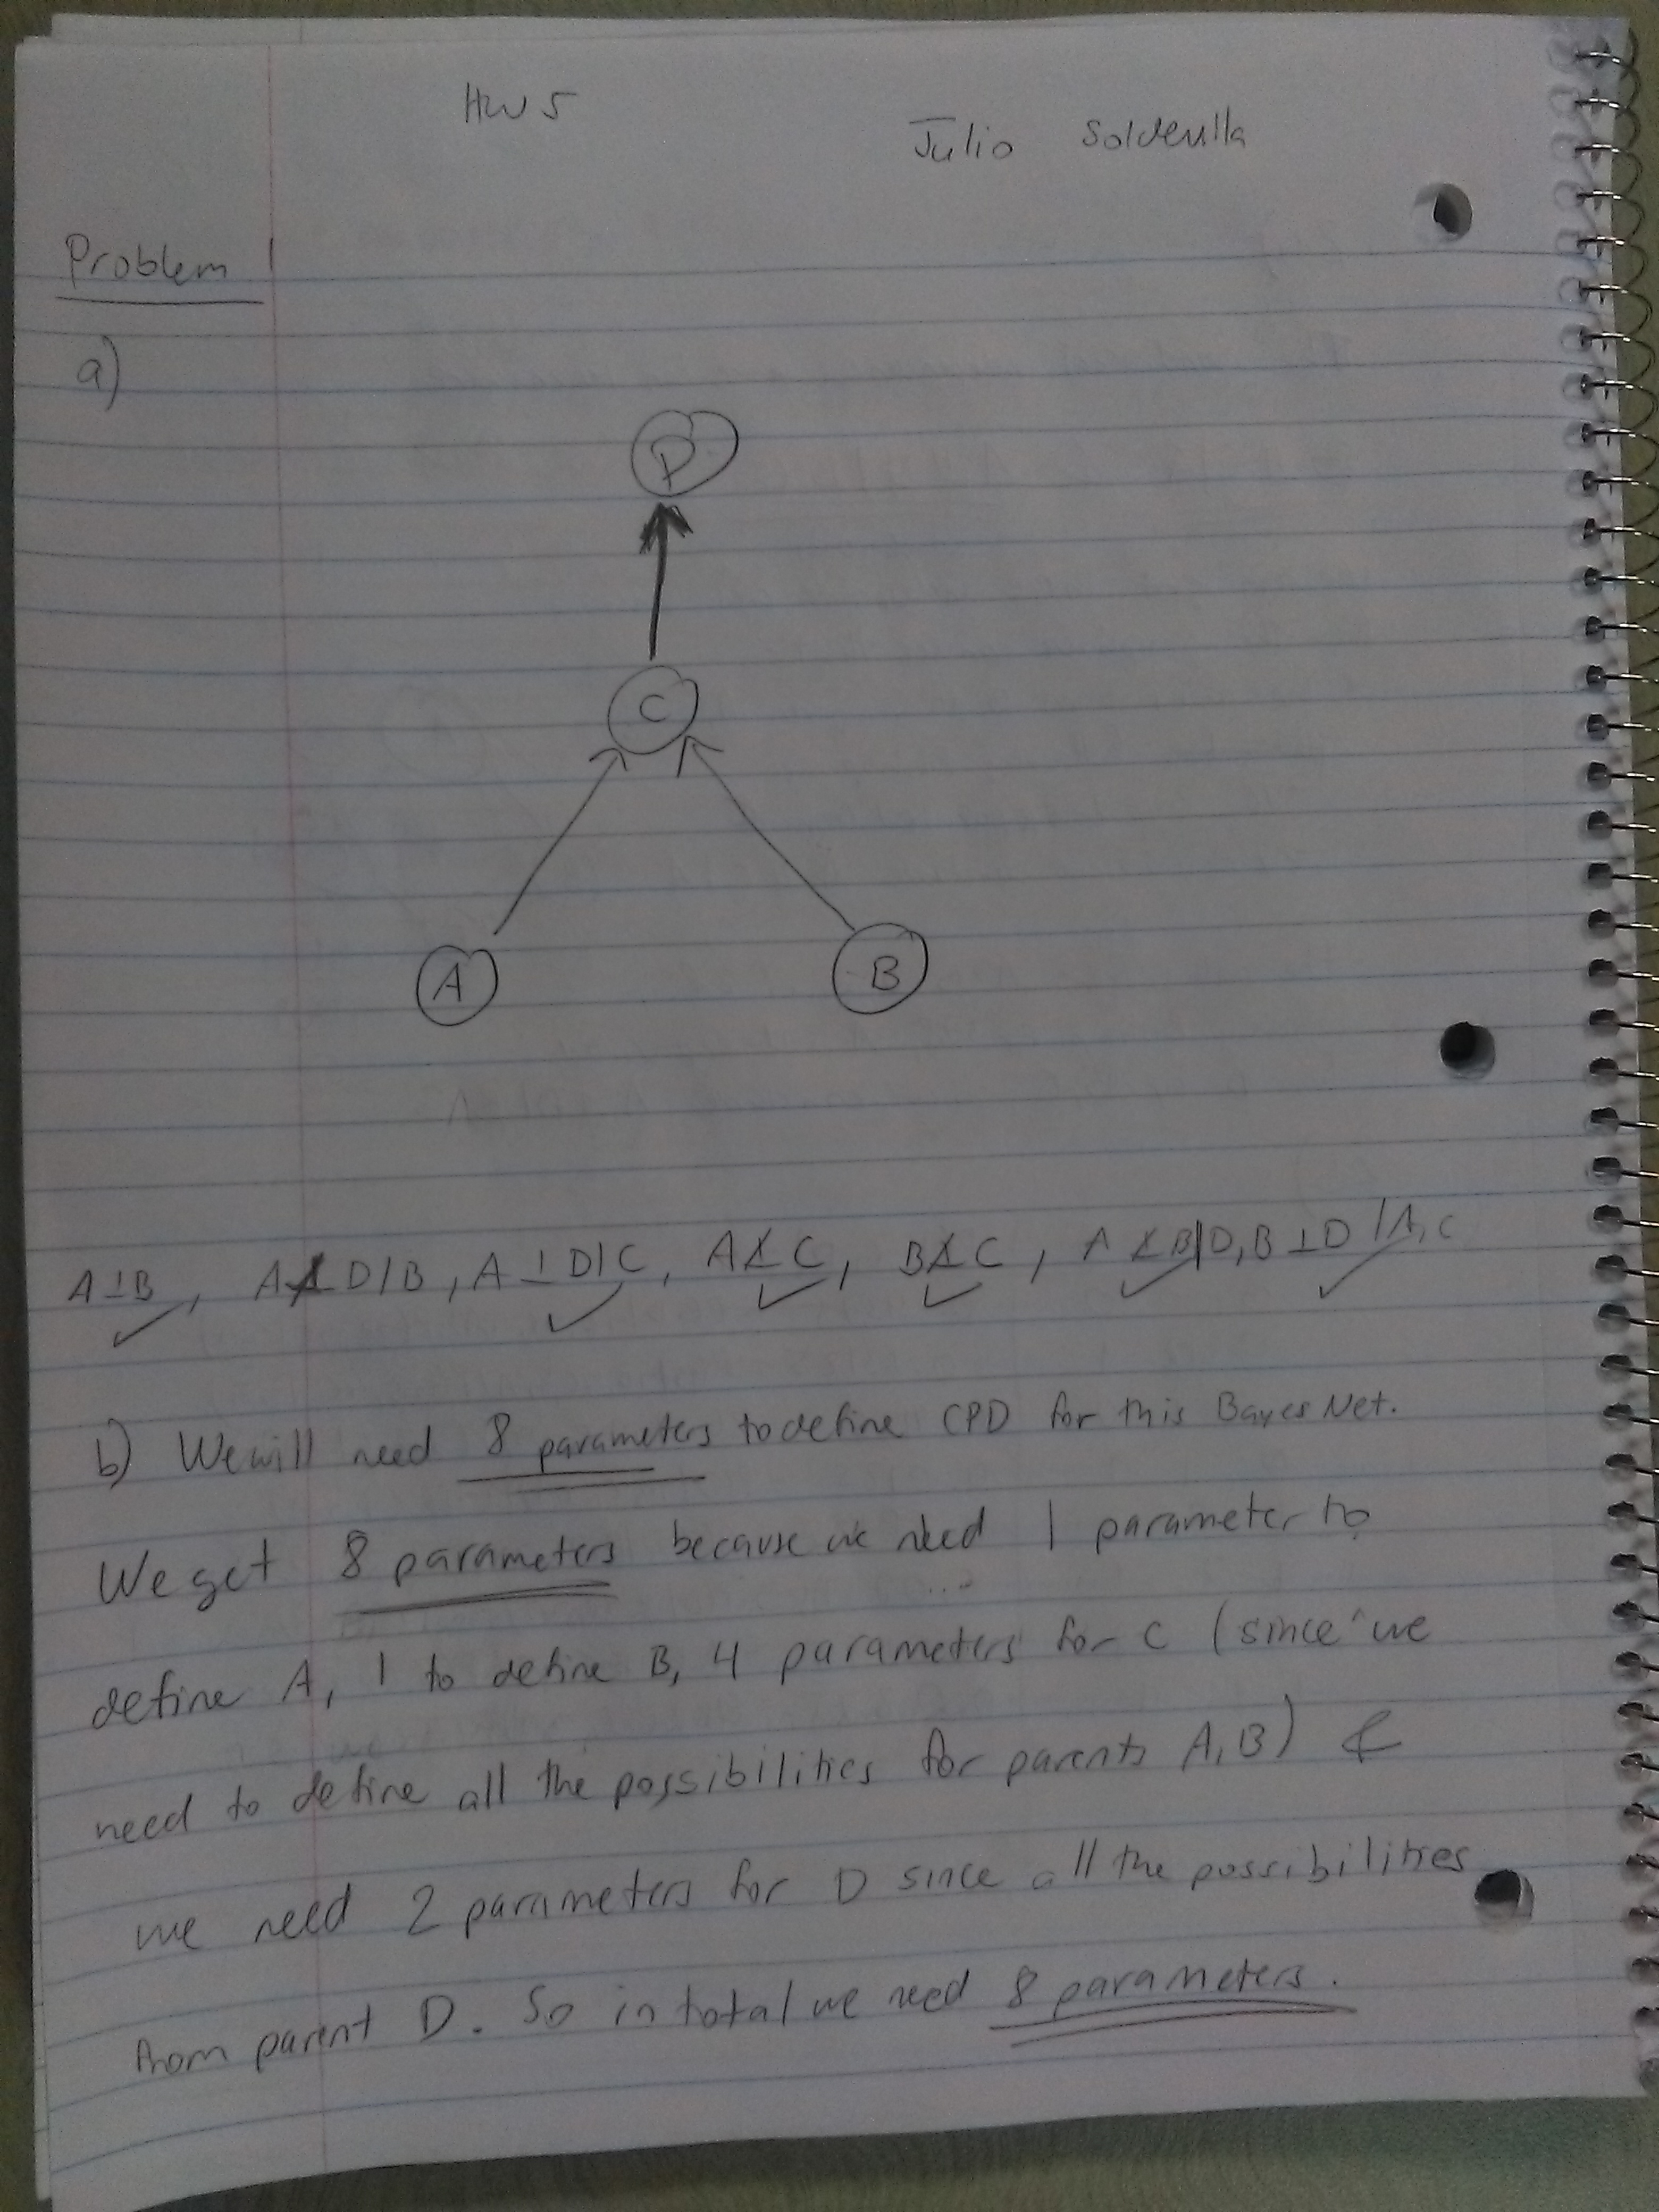
\includegraphics[width = 13cm]{prob1_hw5.jpg}
\caption{\textbf{Problem 1 part a and b:} Image showing the work for part a and b of problem 1}
\end{figure}

\end{proof}

\newpage
\begin{problem}
\normalfont 
Problem 2
\end{problem}

\begin{proof}

\begin{figure}[!htbp]
\centering
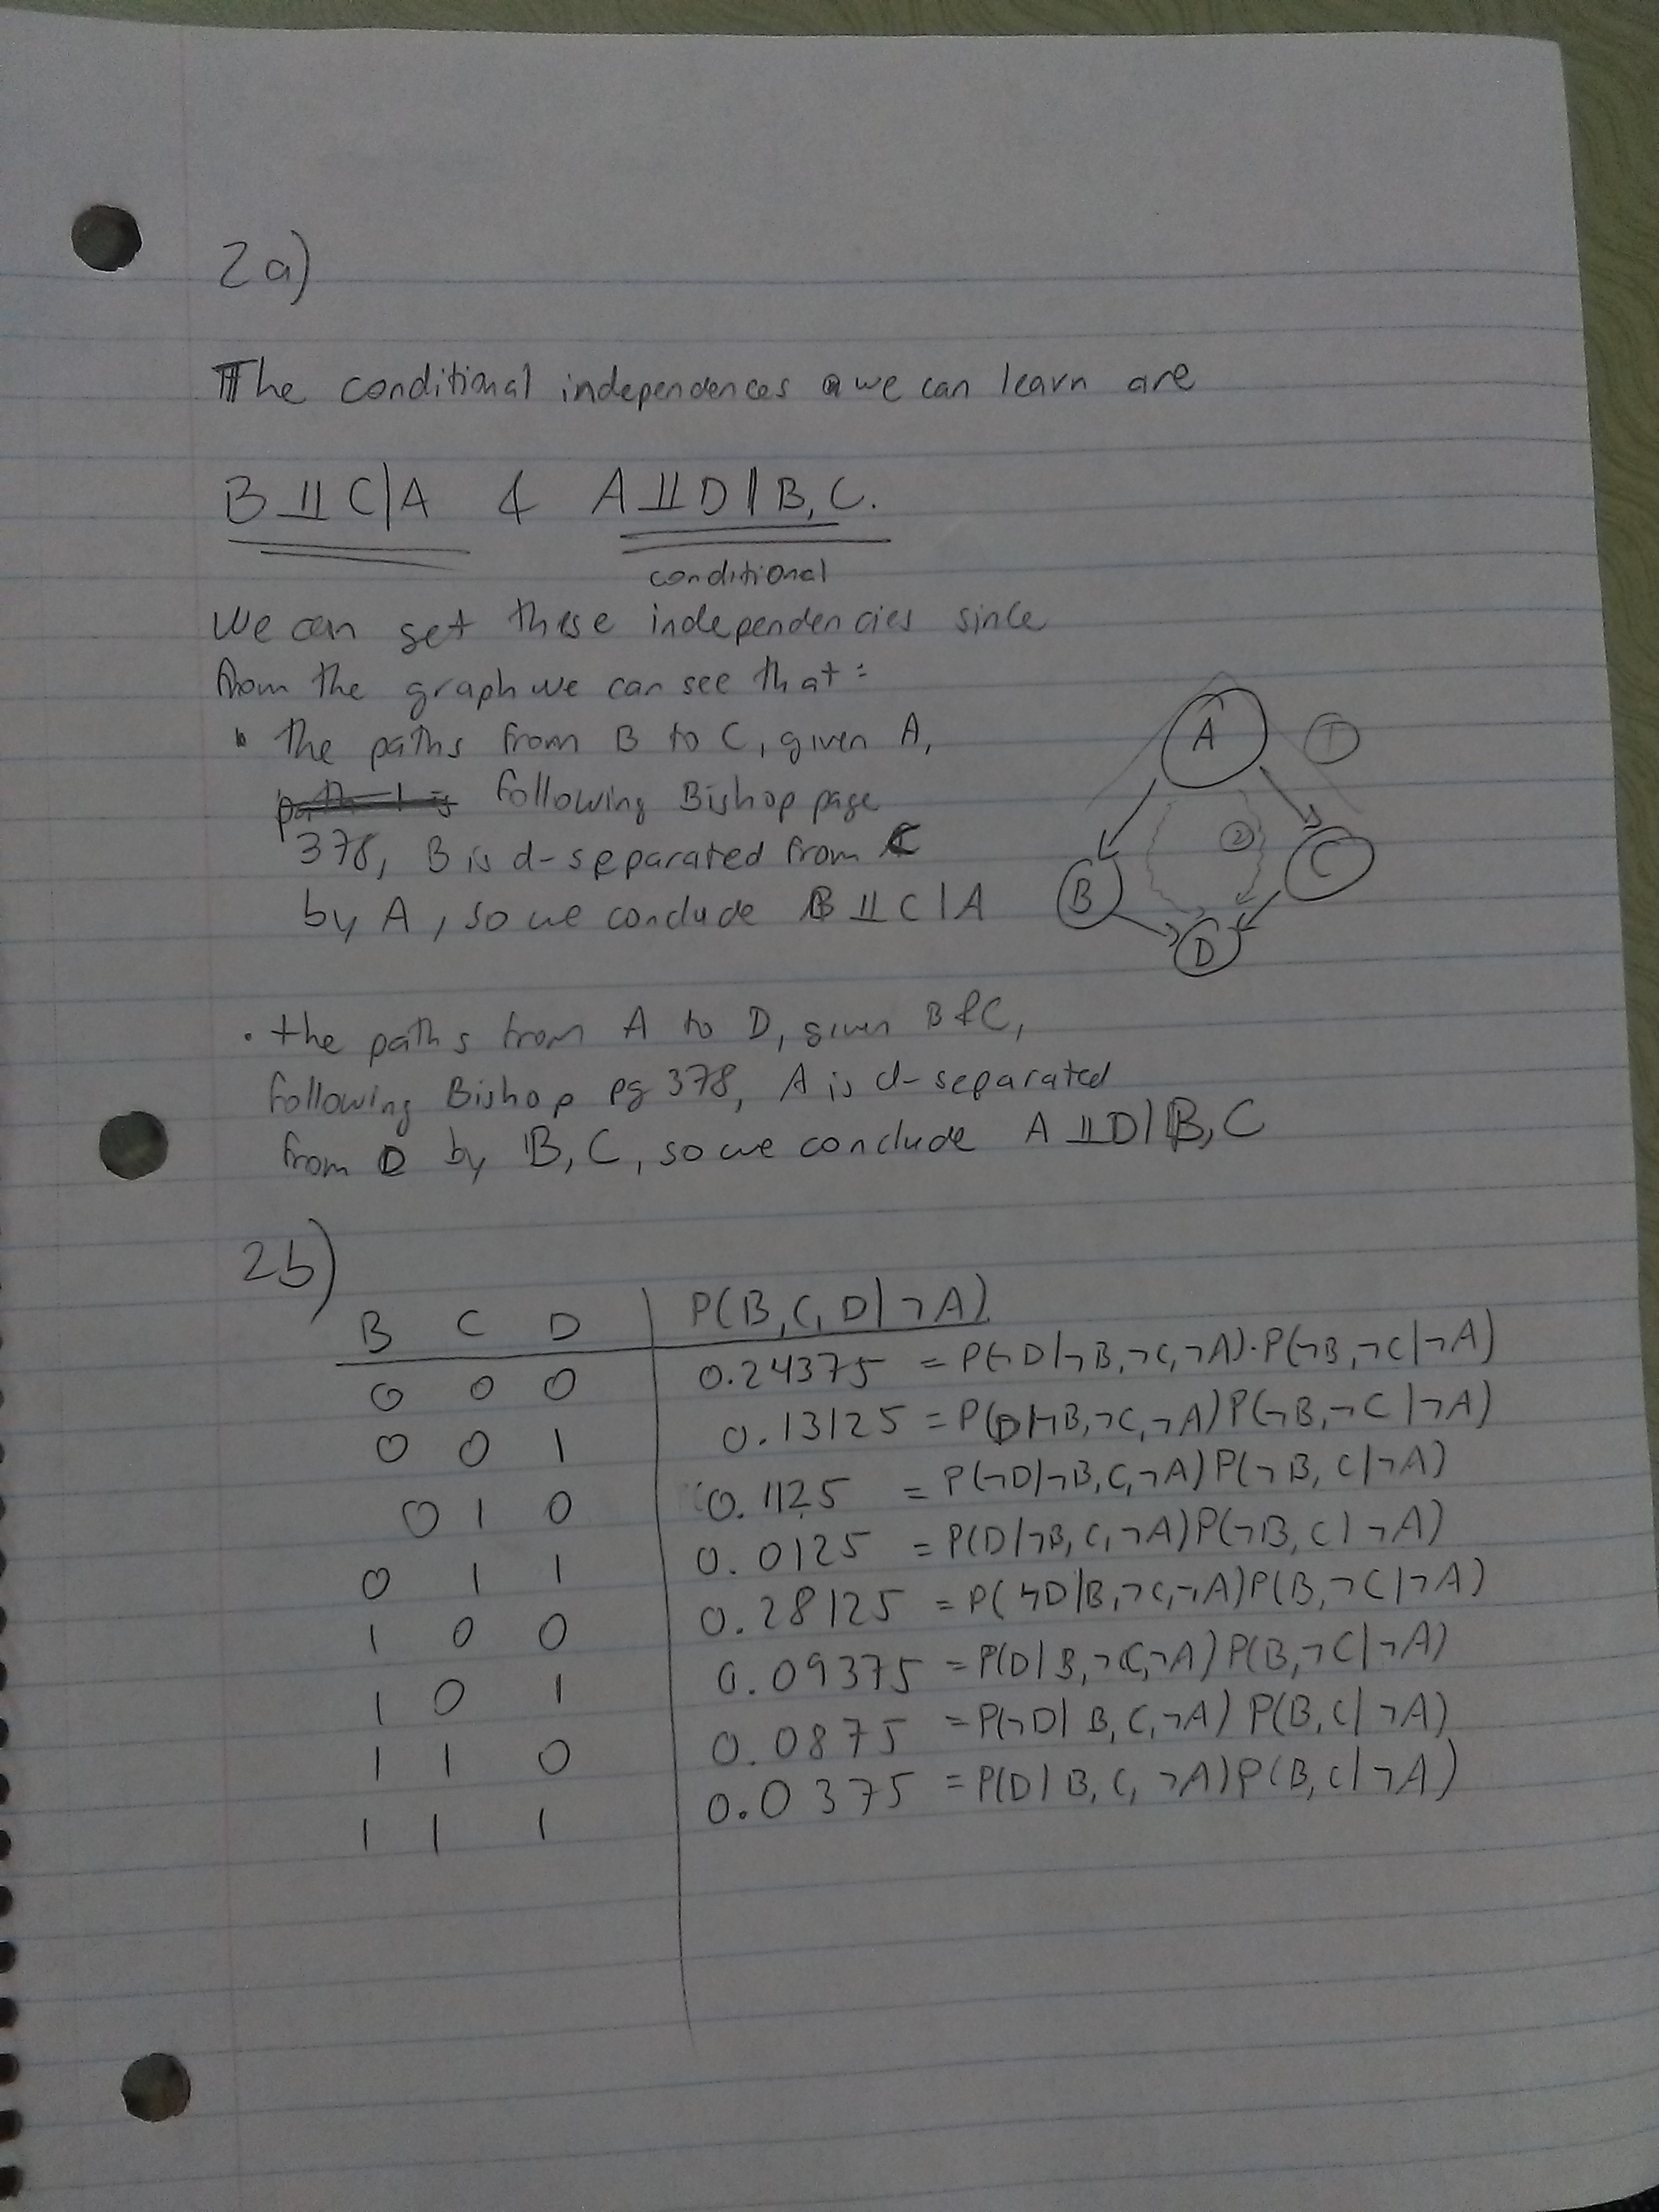
\includegraphics[width = 13cm]{prob2_hw5.jpg}
\caption{\textbf{Problem 2 part a and b:} Image showing the work for part a and b of problem 2}
\end{figure}

\end{proof}

\newpage
\begin{problem}
\normalfont 
Problem 3
\end{problem}

\begin{proof}

\begin{figure}[!htbp]
\centering
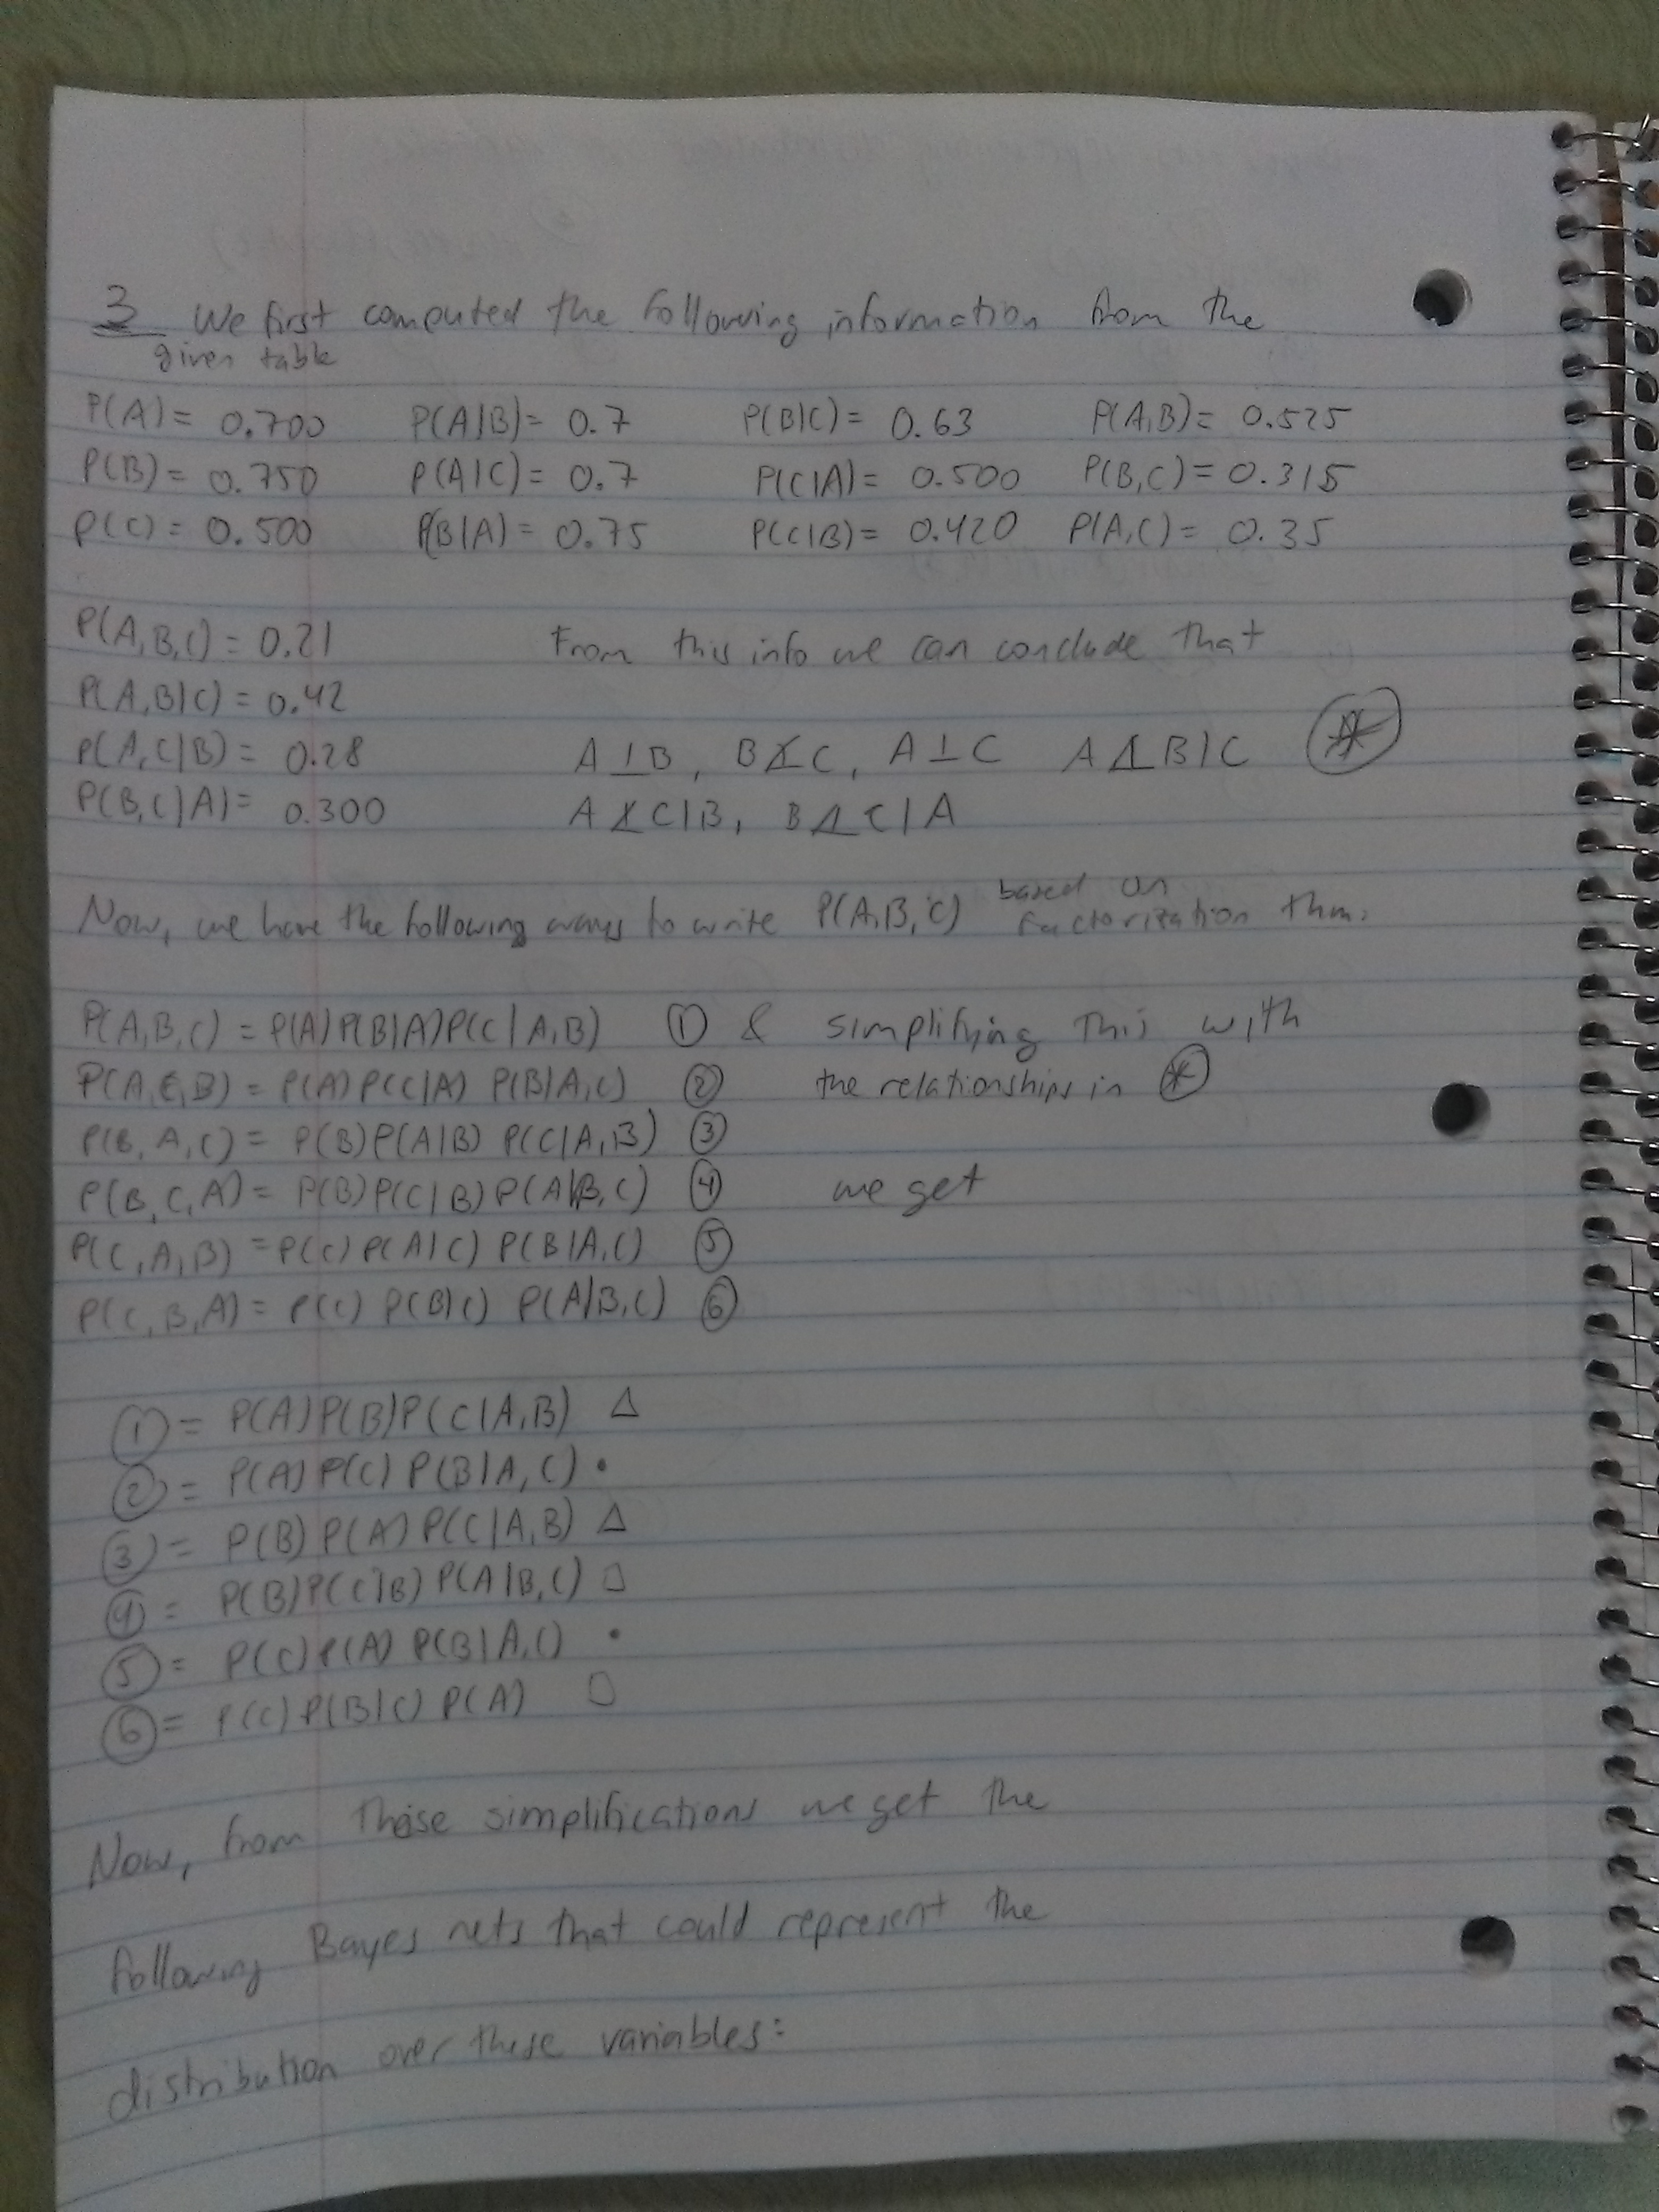
\includegraphics[width = 13cm]{prob3_hw5.jpg}
\caption{\textbf{Problem 3} Image showing the work for problem 3}
\end{figure}

\begin{figure}[!htbp]
\centering
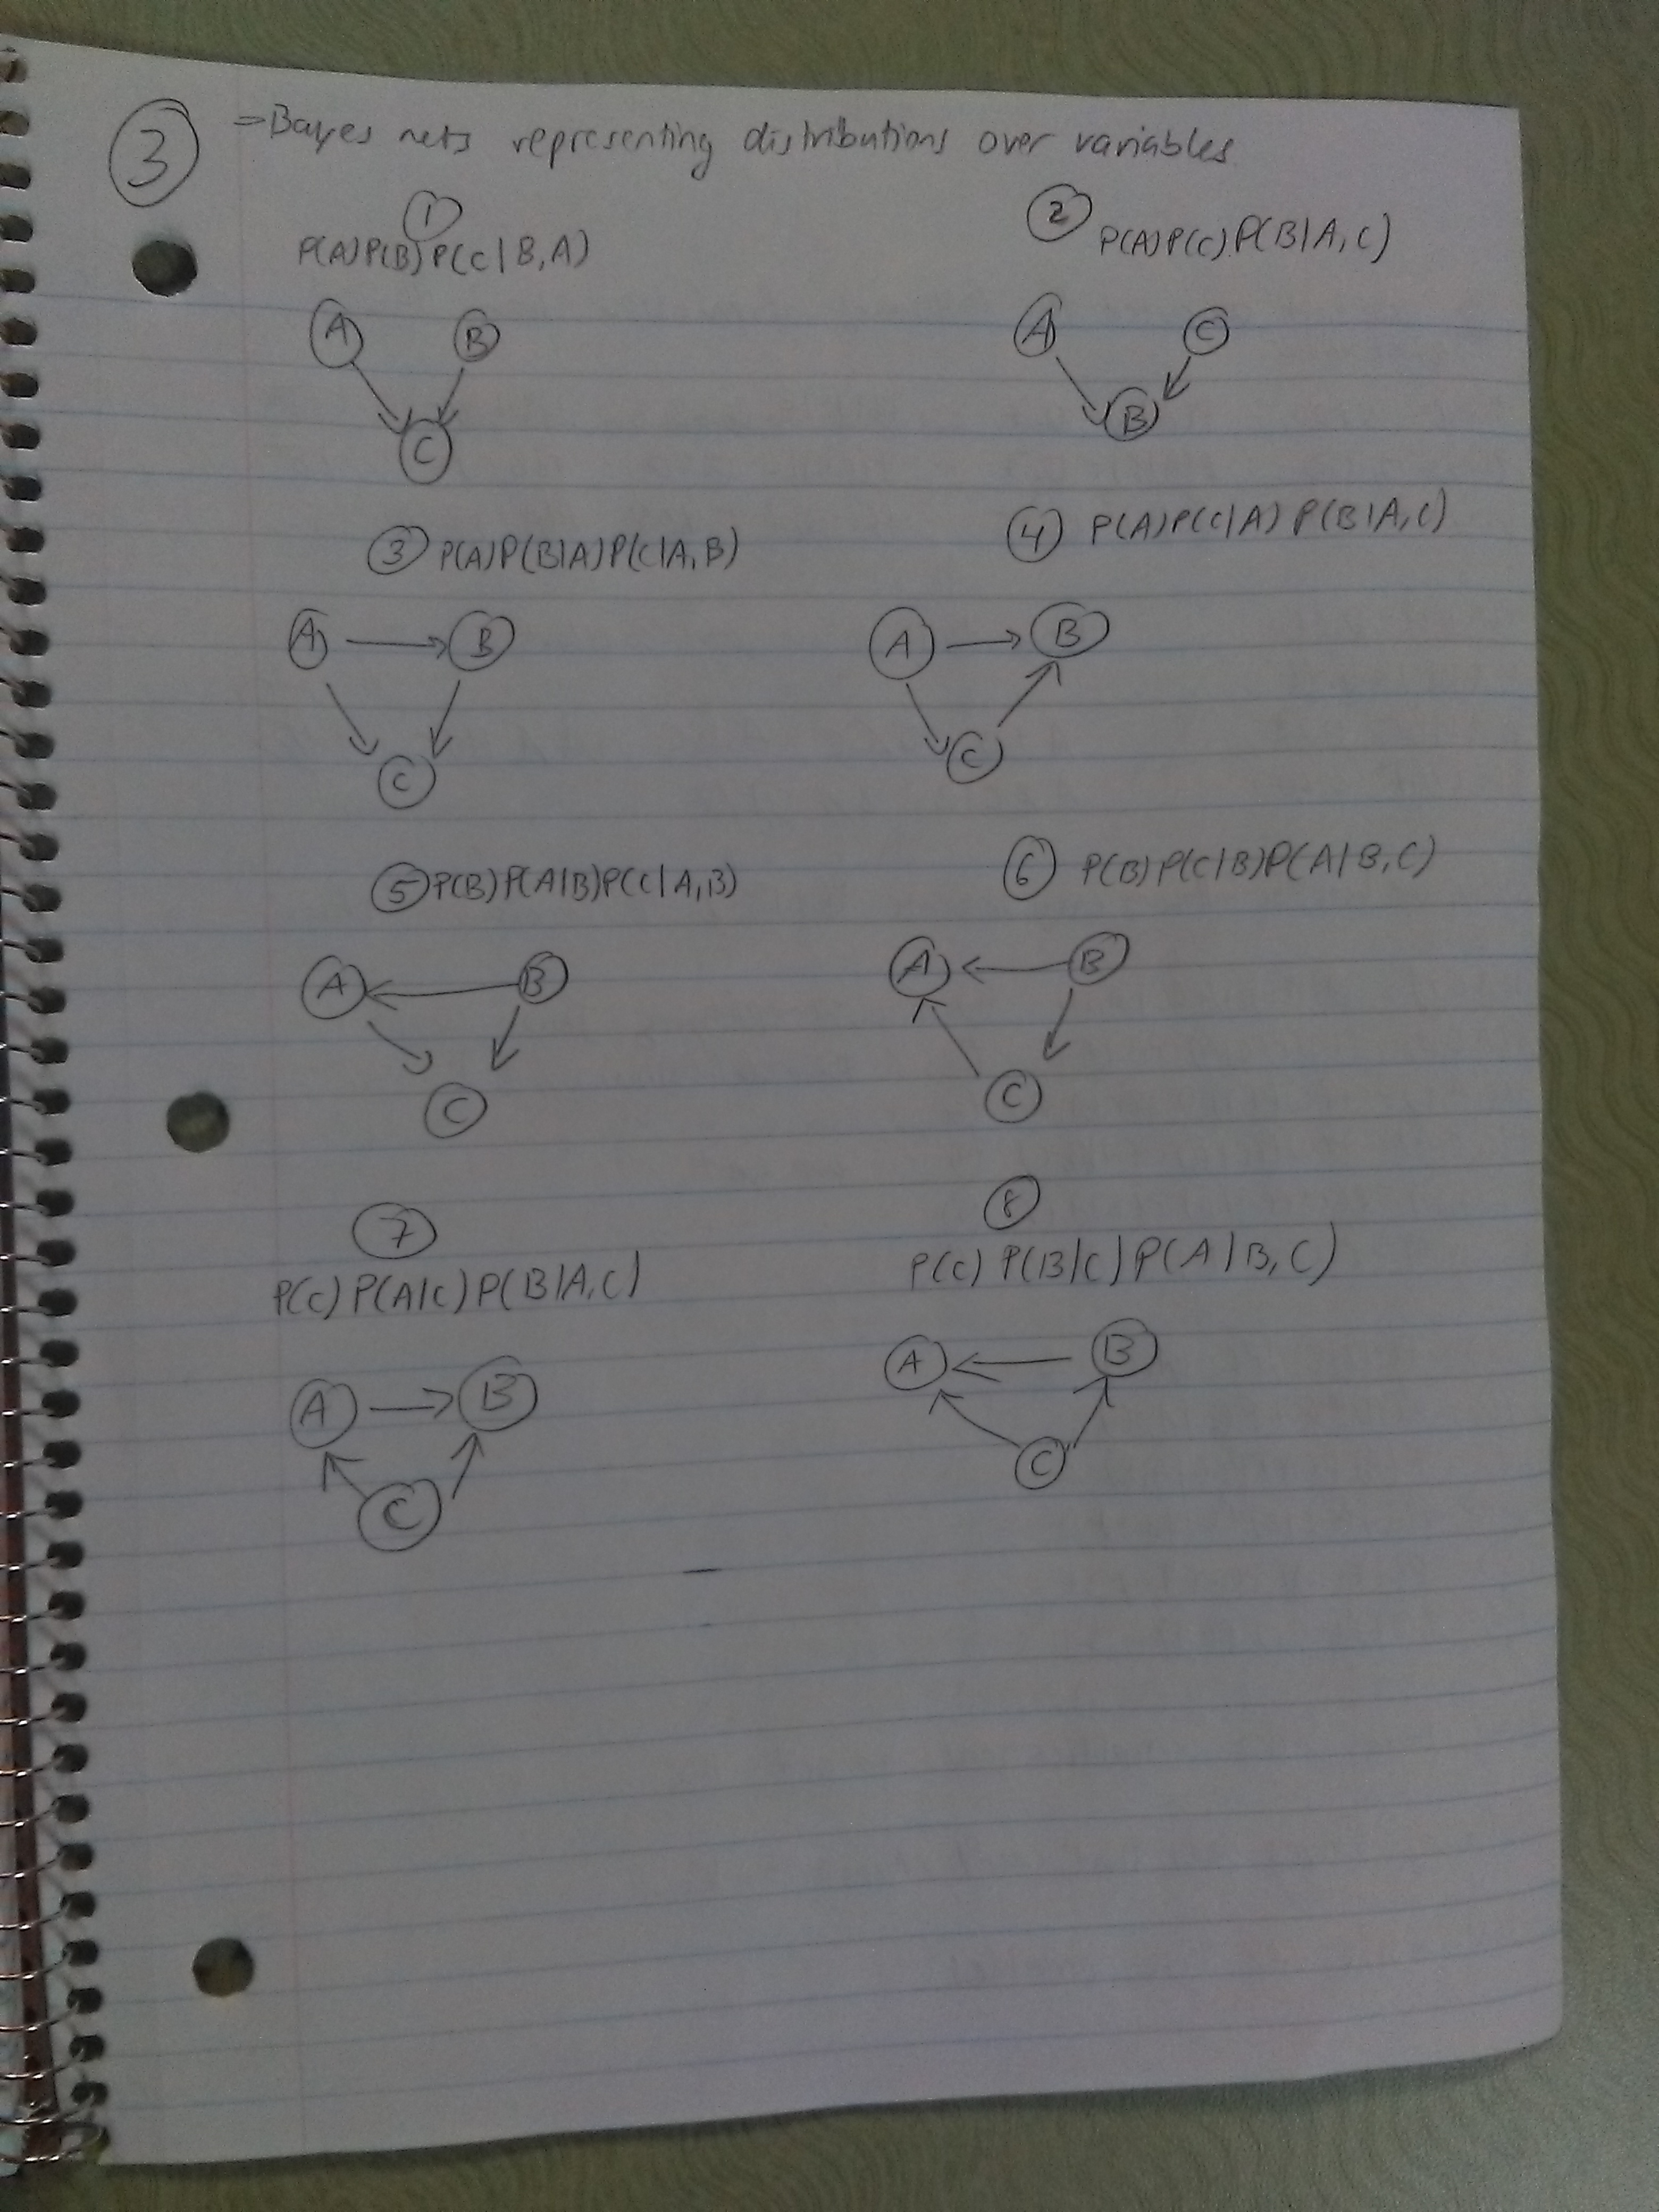
\includegraphics[width = 13cm]{prob3_2_hw5.jpg}
\caption{\textbf{Problem 3} Image showing the work for problem 3}
\end{figure}

\end{proof}

\newpage
\newpage

\begin{problem}
\normalfont 
Problem 4
\end{problem}

\begin{proof}

\begin{enumerate}

\item For the first part of this problem, we see, in the following graph, the picture of the scatter plot of the data.

\begin{figure}[!htbp]
\centering
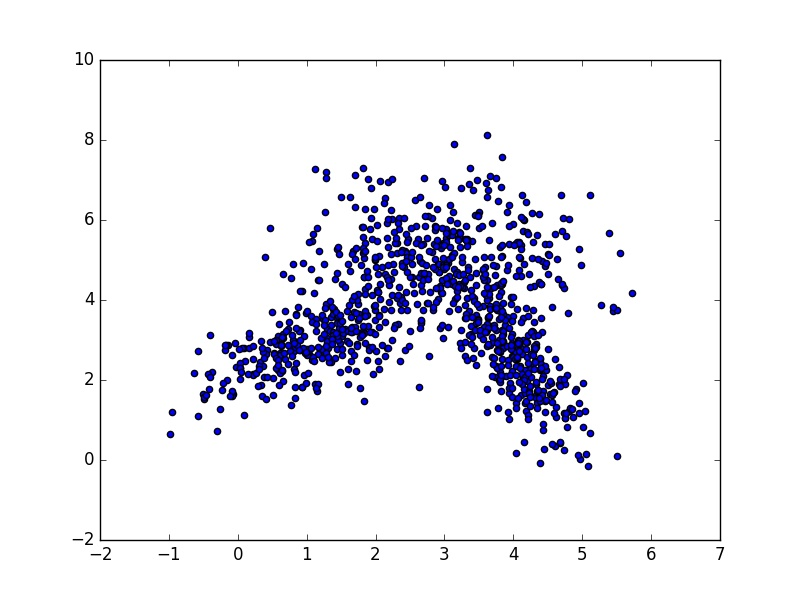
\includegraphics[width = 10cm]{prob4_scatter.jpg}
\caption{\textbf{Problem 4a} Image showing the scatter plot for problem 4}
\end{figure}

Now, when we have $K = 2$, we get the following Gaussian components in the mixture: with mean $\mu = \left\{ \left[ \begin{matrix} 1.49386365 \\3.60593399 \end{matrix} \right] \left[ \begin{matrix} 3.74590611 \\ 3.68496211 \end{matrix}\right] \right\}$ and the covariance matrices $\Sigma = \left\{ \left[ \begin{matrix} 0.98615571 & 0.90483046 \\  0.90483046 & 1.61666384 \end{matrix} \right], \left[ \begin{matrix} 0.56267209 & -0.71849557 \\  -0.71849557 & 2.81343664 \end{matrix} \right] \right\}$ and we get the following scatter plot with the clusters. \\

\begin{figure}[!htbp]
\centering
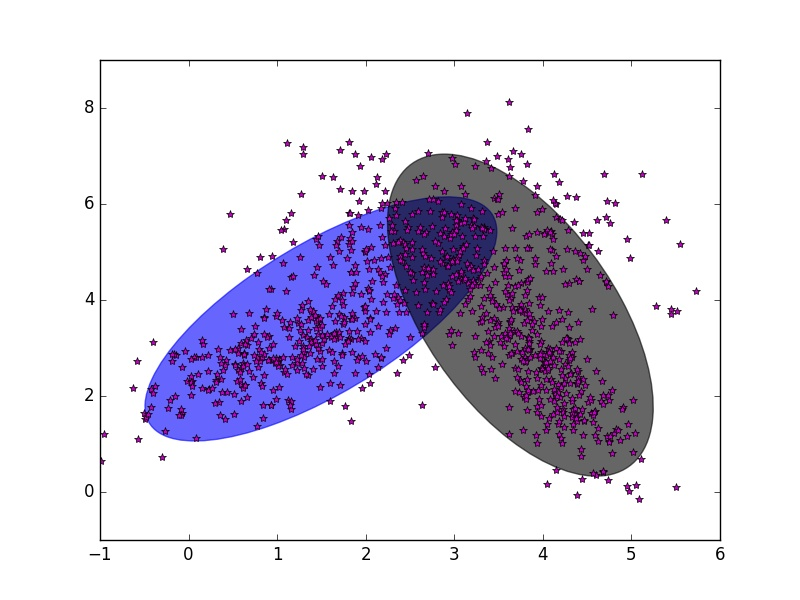
\includegraphics[width = 10cm]{prob4a_k2.jpg}
\caption{\textbf{Problem 4a} Image showing the scatter plot and result of EM algorithm for 2 clusters.}
\end{figure}

Now, when we have $K = 3$, we get the following Gaussian components in the mixture: with mean $\mu = \left\{ \left[ \begin{matrix} 1.08271327 \\ 2.8828234 \end{matrix} \right] \left[ \begin{matrix} 2.97193003 \\ 5.04472742 \end{matrix}\right] \left[ \begin{matrix} 4.04333322 \\ 2.50060083 \end{matrix}\right] \right\}$ and the covariance matrices $\Sigma = \left\{ \left[ \begin{matrix} 0.64506251 & 0.38116334 \\ 0.38116334 & 0.5568736\end{matrix} \right], \left[ \begin{matrix} 1.01331798 & -0.02915437 \\ -0.02915437 & 1.01501022 \end{matrix} \right], \left[ \begin{matrix} 0.21979711 &-0.37026767 \\ -0.37026767 & 1.14190251 \end{matrix} \right] \right\}$ and we get the following scatter plot with the clusters. \\

\begin{figure}[!htbp]
\centering
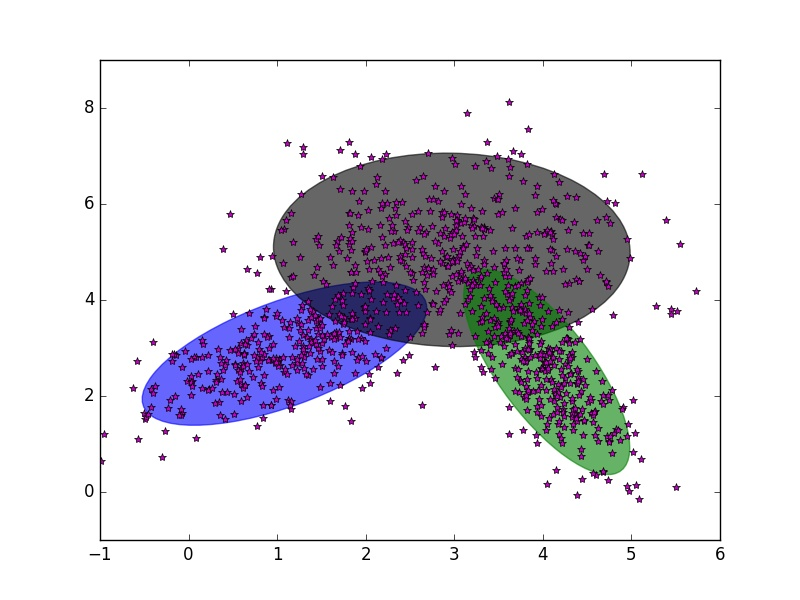
\includegraphics[width = 10cm]{prob4a_k3.jpg}
\caption{\textbf{Problem 4a} Image showing the scatter plot and result of EM algorithm for 3 clusters.}
\end{figure}

Now, when we have $K = 5$, we get the following Gaussian components in the mixture: with mean $\mu = \left\{ \left[ \begin{matrix} 1.87818858 \\ 2.68555211 \end{matrix} \right] \left[ \begin{matrix} 2.98754896 \\ 5.0617341 \end{matrix}\right] \left[ \begin{matrix} 4.07182365 \\ 2.21736995 \end{matrix}\right],\left[ \begin{matrix} 3.95411976 \\ 3.045238 \end{matrix}\right],\left[ \begin{matrix} 1.01229367 \\ 2.90454076 \end{matrix}\right] \right\}$ and the covariance matrices $\Sigma = \left\{ \left[ \begin{matrix} 0.12519243 & -0.00347678 \\ -0.00347678 & 0.30986251 \end{matrix} \right], \left[ \begin{matrix} 1.01766795 & -0.04941322 \\ -0.04941322 & 0.98578055 \end{matrix} \right], \left[ \begin{matrix} 0.2104126 & -0.32793317 \\ -0.32793317 & 1.00038797 \end{matrix} \right], \right\}$ \\ $ \left\{\left[ \begin{matrix} 0.26025229 & -0.45255172 \\ -0.45255172 & 1.03764694 \end{matrix} \right],\left[ \begin{matrix} 0.61327566 & 0.42382975 \\ 0.42382975 & 0.58797768 \end{matrix} \right] \right\}$ and we get the following scatter plot with the clusters.\\

\begin{figure}[!htbp]
\centering
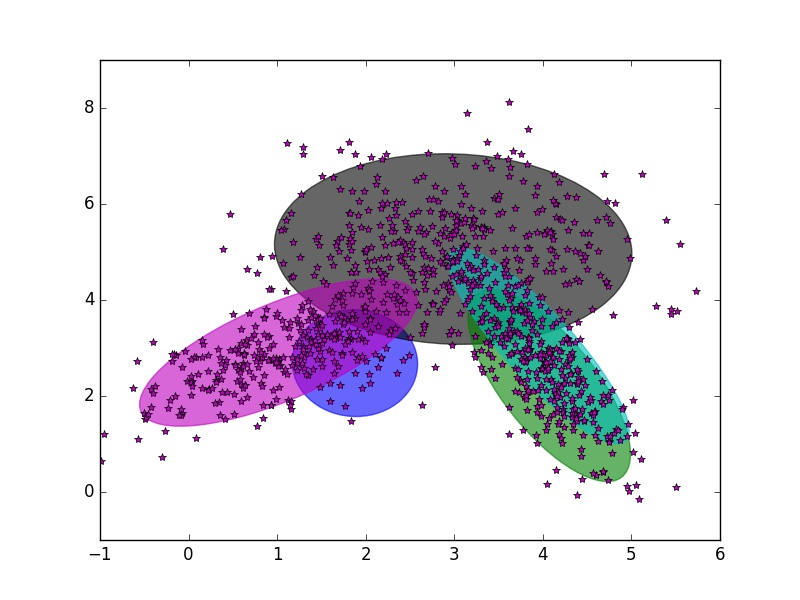
\includegraphics[width = 10cm]{prob4a_k5.jpg}
\caption{\textbf{Problem 4a} Image showing the scatter plot and result of EM algorithm for 5 clusters.}
\end{figure}

Now, when we have $K = 10$, we get the following Gaussian components in the mixture: with mean $\mu = \left\{ \left[ \begin{matrix} 3.6025199 \\ 4.83936943 \end{matrix} \right] \left[ \begin{matrix} 4.71296034 \\ 0.1986524 \end{matrix}\right] \left[ \begin{matrix} 4.356082 \\ 1.6782708  \end{matrix}\right],\left[ \begin{matrix} 4.12471251 \\ 2.85796  \end{matrix}\right],\left[ \begin{matrix} 2.14465053 \\ 5.08194636 \end{matrix}\right],\left[ \begin{matrix} 3.85398589 \\ 2.10096814 \end{matrix}\right], \right\}$ $\left\{ \left[ \begin{matrix} 3.75209835 \\ 3.20487639 \end{matrix}\right],\left[ \begin{matrix} 1.30307196 \\ 3.29183234 \end{matrix}\right],\left[ \begin{matrix} 1.14010914 \\ 2.78515828 \end{matrix}\right],\left[ \begin{matrix} 3.4274561 \\ 5.20456023 \end{matrix}\right] \right\}$ and the covariance matrices \\
 $\Sigma = \left\{ \left[ \begin{matrix} 3.75429517e-01 & 4.41361567e-01 \\ 4.41361567e-01 & 5.19969327e-01 \end{matrix} \right], \left[ \begin{matrix} 1.48798492e-01 & -2.85454354e-02 \\ -2.85454354e-02 & 3.49132323e-02\end{matrix} \right] \right\}$ $\left\{ \left[ \begin{matrix} 1.22727443e-01 & -6.60134578e-02 \\ -6.60134578e-02 & 2.50033836e-01 \end{matrix} \right],\left[ \begin{matrix} 1.99033468e-02 & 2.84515021e-02 \\ 2.84515021e-02 & 6.58684882e-02 \end{matrix} \right], \right\}$ $\left\{ \left[ \begin{matrix} 6.25215337e-01 & 2.66846671e-01 \\ 2.66846671e-01 & 1.14271145e+00 \end{matrix} \right], \left[ \begin{matrix} 1.35135357e-02 & 1.58503668e-03 \\ 1.58503668e-03 & 2.50685466e-04 \end{matrix} \right],\right\}$ $\left\{\left[ \begin{matrix} 2.08282963e-01 & -3.02666524e-01 \\ -3.02666524e-01 & 8.50492621e-01\end{matrix} \right],\left[ \begin{matrix} 1.00560907e+00 & 9.90227009e-01 \\ 9.90227009e-01 & 1.14660462e+00\end{matrix} \right],\right\}$ $\left\{\left[ \begin{matrix} 6.58828033e-01 & 2.24299843e-01 \\ 2.24299843e-01 & 3.91589498e-01 \end{matrix} \right],\left[ \begin{matrix} 8.85017840e-01 & -1.96596216e-01 \\ -1.96596216e-01 & 8.51715398e-01 \end{matrix} \right] \right\}$ and we get the following scatter plot with the clusters.\\


\begin{figure}[!htbp]
\centering
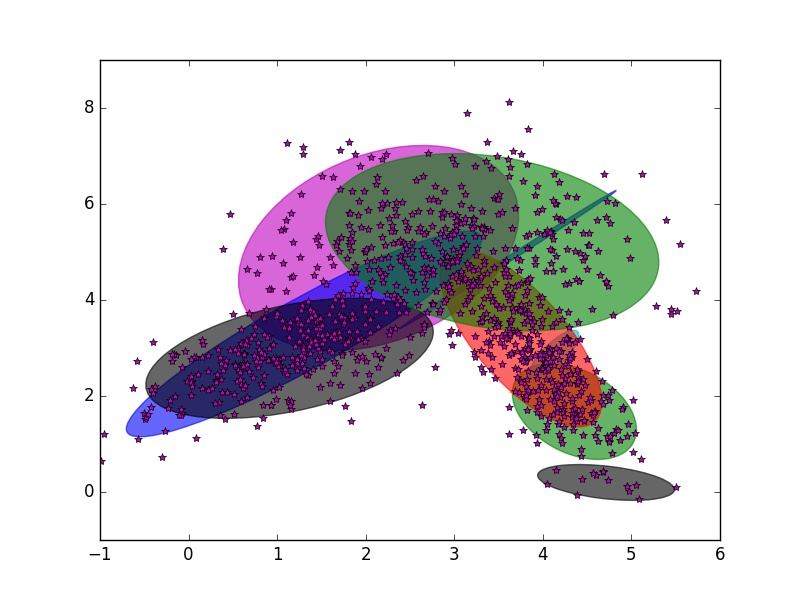
\includegraphics[width = 10cm]{prob4a_k10.jpg}
\caption{\textbf{Problem 4a} Image showing the scatter plot and result of EM algorithm for 10 clusters.}
\end{figure}

\newpage

\item Now, in this problem, we perform the EM algorithm and plot the results after 1,5, 10, 20 and 50 steps. We get the following graphs:

\begin{figure}[!htbp]
\centering
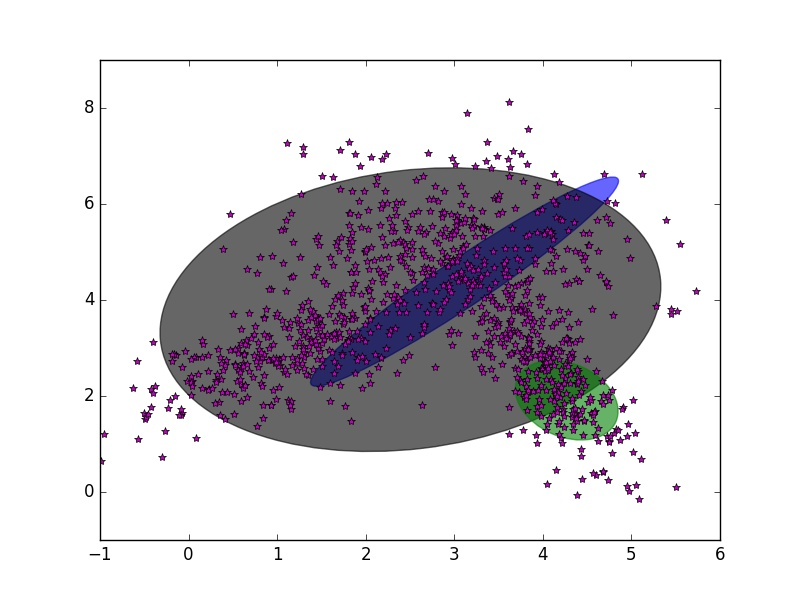
\includegraphics[width = 10cm]{prob4b_1.jpg}
\caption{\textbf{Problem 4b} Image showing the EM algorithm result after 1 step of the algorithm}
\end{figure}

\begin{figure}[!htbp]
\centering
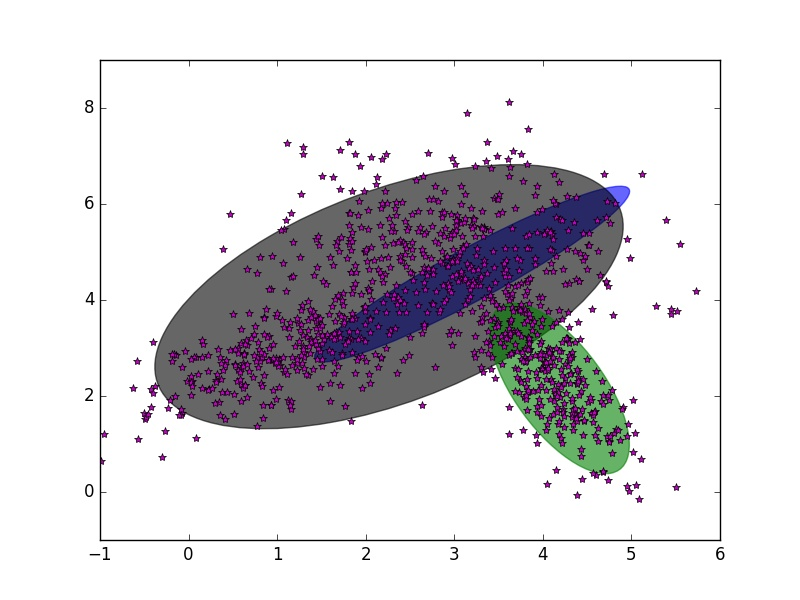
\includegraphics[width = 10cm]{prob4b_5.jpg}
\caption{\textbf{Problem 4b} Image showing the EM algorithm result after 5 step of the algorithm}
\end{figure}

\begin{figure}[!htbp]
\centering
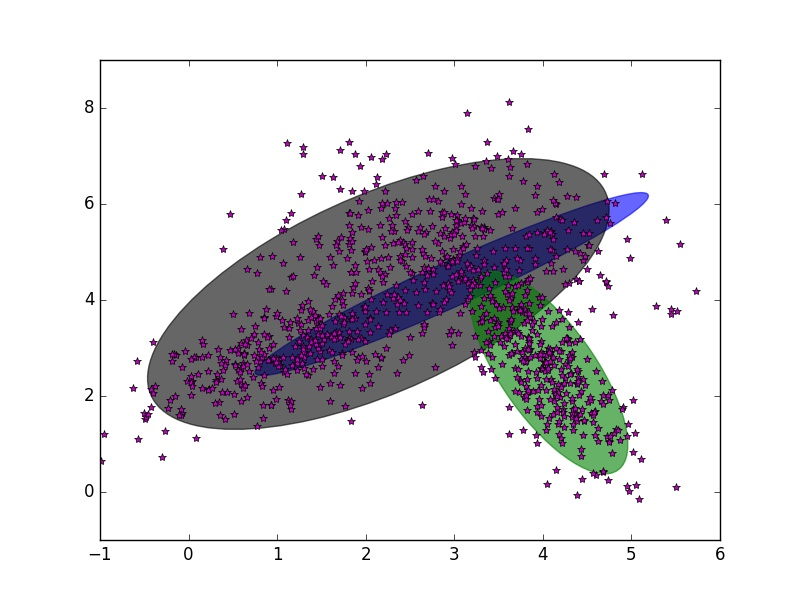
\includegraphics[width = 10cm]{prob4b_10.jpg}
\caption{\textbf{Problem 4b} Image showing the EM algorithm result after 10 step of the algorithm}
\end{figure}

\begin{figure}[!htbp]
\centering
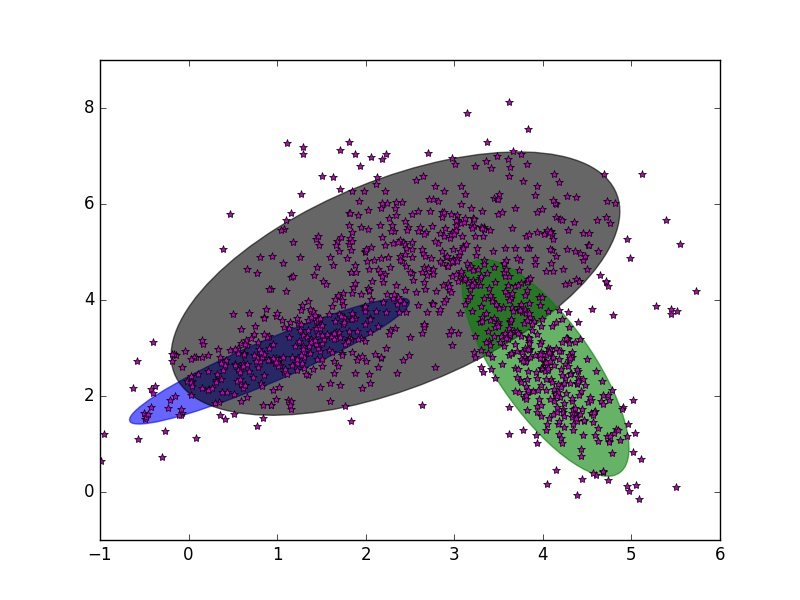
\includegraphics[width = 10cm]{prob4b_20.jpg}
\caption{\textbf{Problem 4b} Image showing the EM algorithm result after 20 step of the algorithm}
\end{figure}

\begin{figure}[!htbp]
\centering
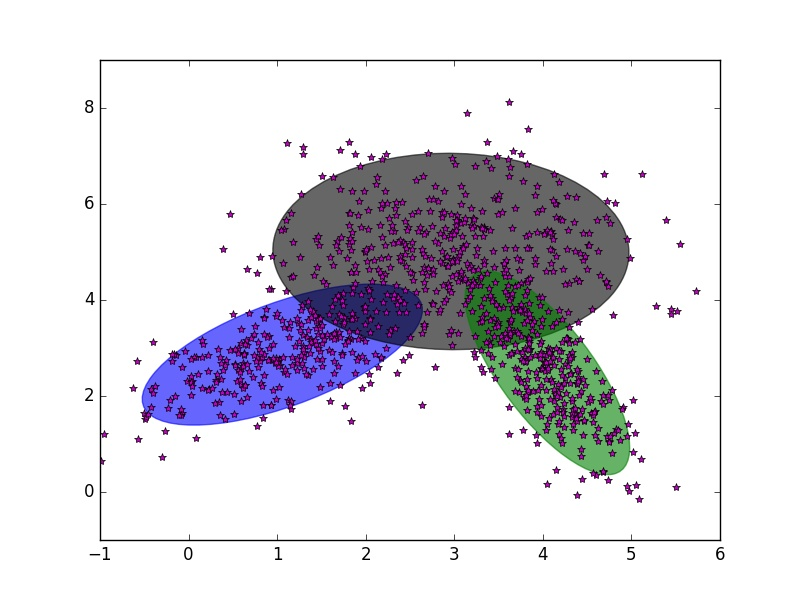
\includegraphics[width = 10cm]{prob4b_50.jpg}
\caption{\textbf{Problem 4b} Image showing the EM algorithm result after 50 step of the algorithm}
\end{figure}

\newpage
\newpage

\item Finally, after playing around with the initialization parameters (particularly) changing the mean, we end up having that 

\begin{figure}[!htbp]
\centering
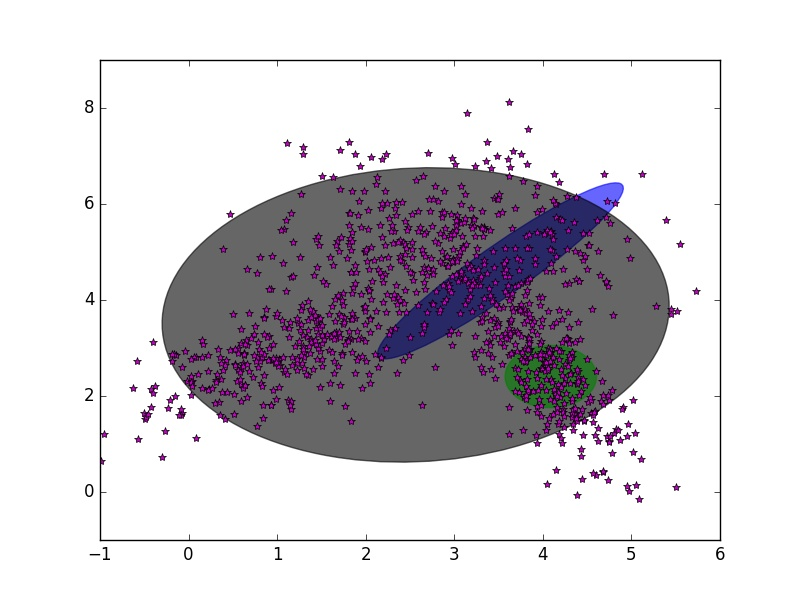
\includegraphics[width = 10cm]{prob4c_1_random_2.jpg}
\caption{\textbf{Problem 4c} Image showing the EM algorithm result after 1 step of the algorithm}
\end{figure}

\begin{figure}[!htbp]
\centering
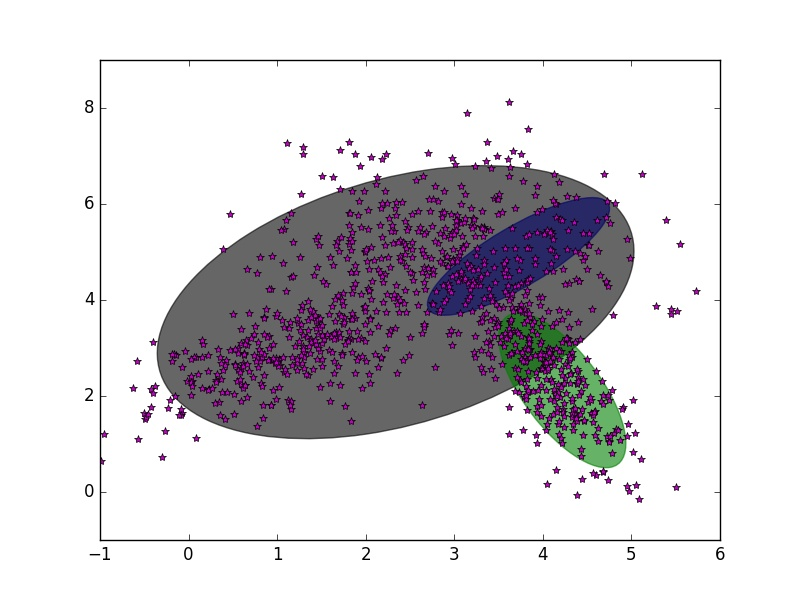
\includegraphics[width = 10cm]{prob4c_5_random_2.jpg}
\caption{\textbf{Problem 4c} Image showing the EM algorithm result after 5 step of the algorithm}
\end{figure}

\begin{figure}[!htbp]
\centering
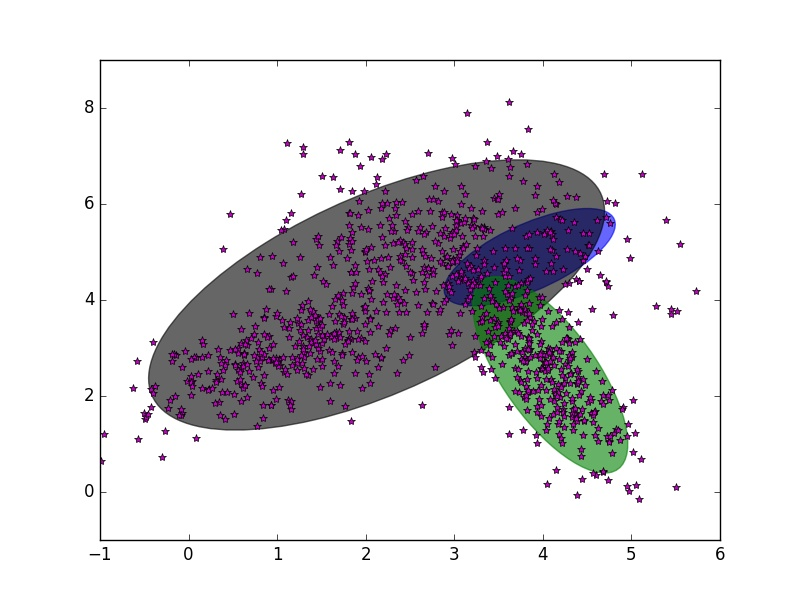
\includegraphics[width = 10cm]{prob4c_10_random_2.jpg}
\caption{\textbf{Problem 4c} Image showing the EM algorithm result after 10 step of the algorithm}
\end{figure}

\begin{figure}[!htbp]
\centering
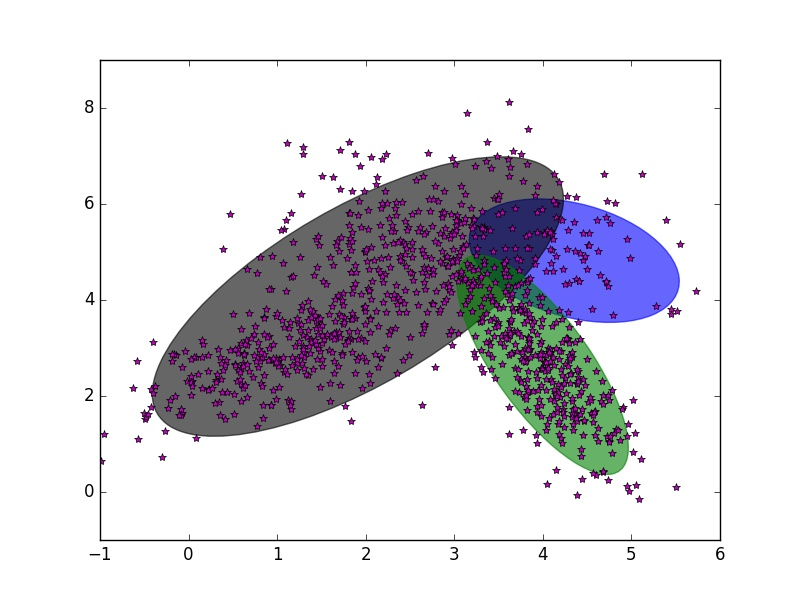
\includegraphics[width = 10cm]{prob4c_20_random_2.jpg}
\caption{\textbf{Problem 4c} Image showing the EM algorithm result after 20 step of the algorithm}
\end{figure}

\begin{figure}[!htbp]
\centering
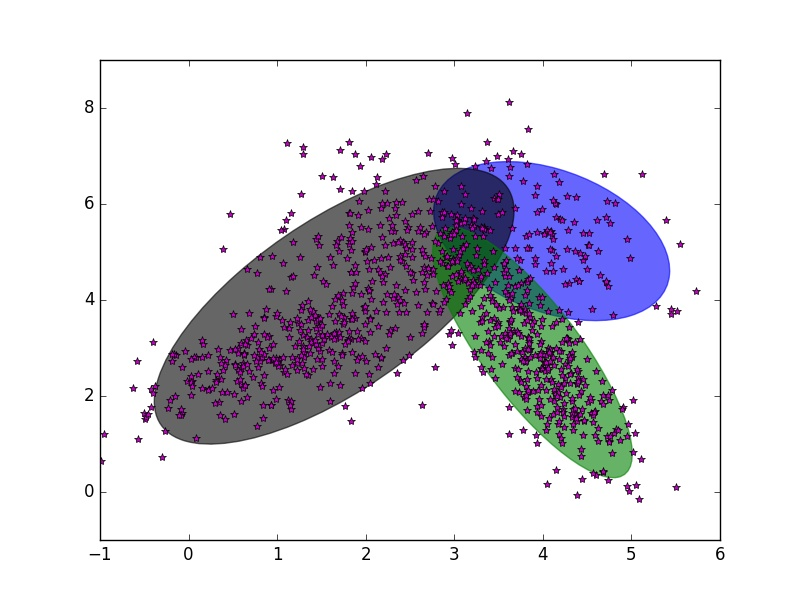
\includegraphics[width = 10cm]{prob4c_50_random_2.jpg}
\caption{\textbf{Problem 4c} Image showing the EM algorithm result after 50 step of the algorithm}
\end{figure}

From these pictures, we see that after changing the initial mean of the EM algorithm, the algorithm learned different clusters that don't quite align with the given data, we are finding clusters centered at different points of the learning space. Also, (not presented in pictures) if we change the initial covariance matrices drastically, the algorithm would learn perhaps thinner or much fatter regions, corresponding to the change in initial covariance.

\end{enumerate}

\end{proof}

\end{document}